% 17-17 ⑵(본책 17쪽) — 가로 4칸·세로 3칸 도로망에서 가운데 가로줄 사이의 세로 도로 한 칸(왼쪽에서 둘째 세로줄·가운데 띠)이 없는 그림. A 왼쪽 위 · B 오른쪽 아래. 스캔 그림을 TikZ 로 다시 그림(스캔 화질).
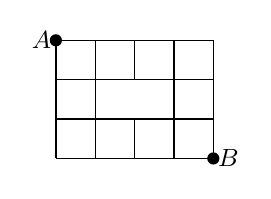
\begin{tikzpicture}[line width=0.5pt]
  \foreach \y in {0, 0.5, 1, 1.5} { \draw (0,\y) -- (2,\y); }
  \foreach \x in {0, 0.5, 1.5, 2} { \draw (\x,0) -- (\x,1.5); }
  \draw (1,0) -- (1,0.5);
  \draw (1,1) -- (1,1.5);
  \fill (0,1.5) circle (2.2pt);
  \node[left, font=\small, inner sep=1.5pt] at (0,1.5) {$\pt{A}$};
  \fill (2,0) circle (2.2pt);
  \node[right, font=\small, inner sep=1.5pt] at (2,0) {$\pt{B}$};
\end{tikzpicture}
